\subsection{Four high-input partitions: ten-minute evaluation}\label{sec:four-partition-updated}
This follow-up kept the 700-message/s total input rate, but concentrated 80\% of the input on four of sixty partitions, initially owned by Consumer 2. The remaining partitions shared the other 20\%. Timing and processing settings matched the twelve-partition comparison. Redistribution within three consumers and scaling to six with targeted redistribution were each tested twice, using workload seeds 81 and 82 and reversing their order in the second repetition. Initial ownership and the original consumer placement were checked. Table~\ref{tab:combined-partition-ownership} gives the final assignments; this follow-up did not include normal Kafka scaling or a no-mitigation run.

Both responses completed all evaluation messages by the drain cutoff. Redistribution within three had lower p99, fewer one-second SLO violations, less backlog and lower resource use in both runs. It also caused shorter processing pauses and confirmed recovery sooner. Tables~\ref{tab:four-partition-outcomes}--\ref{tab:four-partition-intervention-cost} provide the values. Thus, adding consumers did not improve the tested outcomes for this workload. Six consumers retained the earlier scaling setting; this experiment did not establish an optimal consumer count.

For messages produced during the final two evaluation minutes, p99 was 0.187 and 0.349 seconds with redistribution, compared with 2.714 and 0.481 seconds with targeted scaling. All of these messages completed by the drain cutoff. This interval was specified before these trials, unlike the retrospective twelve-partition analysis. The first targeted-scaling run developed another backlog spike after meeting the recovery criterion, showing that an initial recovery does not guarantee continuously low backlog.

Small persistent-hot sets sometimes remained late in these runs despite low absolute backlog. The runtime-state figure therefore needs to be read alongside the absolute lag and growth measurements. Resource integrals use valid observations; per-process CPU coverage was 87.22--99.72\%, interpreted as in Section~\ref{sec:twelve-partition-updated}.

\clearpage
\begingroup
\makeatletter
\setlength{\@fptop}{0pt}
\setlength{\@fpsep}{12pt}
\setlength{\@fpbot}{0pt plus 1fil}
\makeatother
\begin{table}[!htbp]
\centering\small
\setlength{\tabcolsep}{3pt}
\renewcommand{\arraystretch}{1.12}
\begin{tabular}{@{}lrrrrrr@{}}
\toprule
Response & Run & \shortstack{Mean latency\\(s)} & \shortstack{p99\\(s)} & \shortstack{Unfinished\\(\%)} & \shortstack{SLO violations\\1 s (\%)} & \shortstack{Useful throughput\\(msg/s)}\\
\midrule
Redistribute 3 & 1 & 10.749 & 84.50 & 0.000 & 26.63 & 730.87\\
Redistribute 3 & 2 & 9.935 & 79.28 & 0.000 & 25.82 & 731.38\\
Targeted scale 6 & 1 & 19.330 & 110.19 & 0.000 & 35.23 & 730.89\\
Targeted scale 6 & 2 & 20.023 & 112.94 & 0.000 & 34.72 & 731.13\\
\bottomrule
\end{tabular}
\caption{Completion outcomes: four high-traffic partitions.}
\label{tab:four-partition-outcomes}\label{tab:four-partition-latency-details}
\end{table}
\begin{table}[!htbp]
\centering\small
\setlength{\tabcolsep}{3pt}
\renewcommand{\arraystretch}{1.12}
\begin{tabular}{@{}lrrrrr@{}}
\toprule
Response & Run & \shortstack{Actual CPU\\(core-s)} & \shortstack{Actual RSS\\(GiB-min)} & \shortstack{Requested CPU\\(core-min)} & \shortstack{Requested memory\\(GiB-min)}\\
\midrule
Redistribute 3 & 1 & 1,006.9 & 2.75 & 72.00 & 36.00\\
Redistribute 3 & 2 & 1,018.7 & 2.72 & 72.00 & 36.00\\
Targeted scale 6 & 1 & 1,301.6 & 4.09 & 136.83 & 68.42\\
Targeted scale 6 & 2 & 1,300.6 & 4.01 & 136.85 & 68.42\\
\bottomrule
\end{tabular}
\caption{Consumer resources: four high-traffic partitions.}
\label{tab:four-partition-resources}
\end{table}
\begin{table}[!htbp]
\centering\small
\setlength{\tabcolsep}{3pt}
\renewcommand{\arraystretch}{1.12}
\begin{tabular}{@{}lrrrrrr@{}}
\toprule
Response & Run & \shortstack{Mean total\\lag} & \shortstack{Maximum\\total backlog} & \shortstack{Lag coverage\\(\%)} & \shortstack{Maximum\\partition lag} & Mean skew\\
\midrule
Redistribute 3 & 1 & 7,296 & 50,879 & 96.3 & 13,509 & 20.56\\
Redistribute 3 & 2 & 6,994 & 50,157 & 97.0 & 12,258 & 20.88\\
Targeted scale 6 & 1 & 12,683 & 66,598 & 95.7 & 15,839 & 23.00\\
Targeted scale 6 & 2 & 12,740 & 70,217 & 95.0 & 16,277 & 22.72\\
\bottomrule
\end{tabular}
\caption{Backlog and lag skew: four high-traffic partitions.}
\label{tab:four-partition-diagnostics}
\end{table}

\begin{table}[!htbp]
\centering\small
\setlength{\tabcolsep}{3pt}
\renewcommand{\arraystretch}{1.12}
\begin{tabular}{@{}lrrrrrr@{}}
\toprule
Response & Run & \shortstack{Decision to\\active (s)} & \shortstack{Global gap\\(s)} & \shortstack{Extra pending\\during pause} & \shortstack{Net pending\\during transfer} & \shortstack{Recovery\\(s)}\\
\midrule
Redistribute 3 & 1 & 27.26 & 15.080 & 10,557 & 7,023 & 180.9\\
Redistribute 3 & 2 & 21.92 & 12.307 & 8,614 & 6,019 & 173.4\\
Targeted scale 6 & 1 & 78.52 & 19.881 & 13,918 & 4,678 & 290.5\\
Targeted scale 6 & 2 & 81.26 & 21.732 & 15,305 & 5,523 & 266.8\\
\bottomrule
\end{tabular}
\caption{Intervention time and recovery: four high-traffic partitions.}
\label{tab:four-partition-intervention-cost}
\end{table}
\clearpage
\begin{figure}[!htbp]
\centering
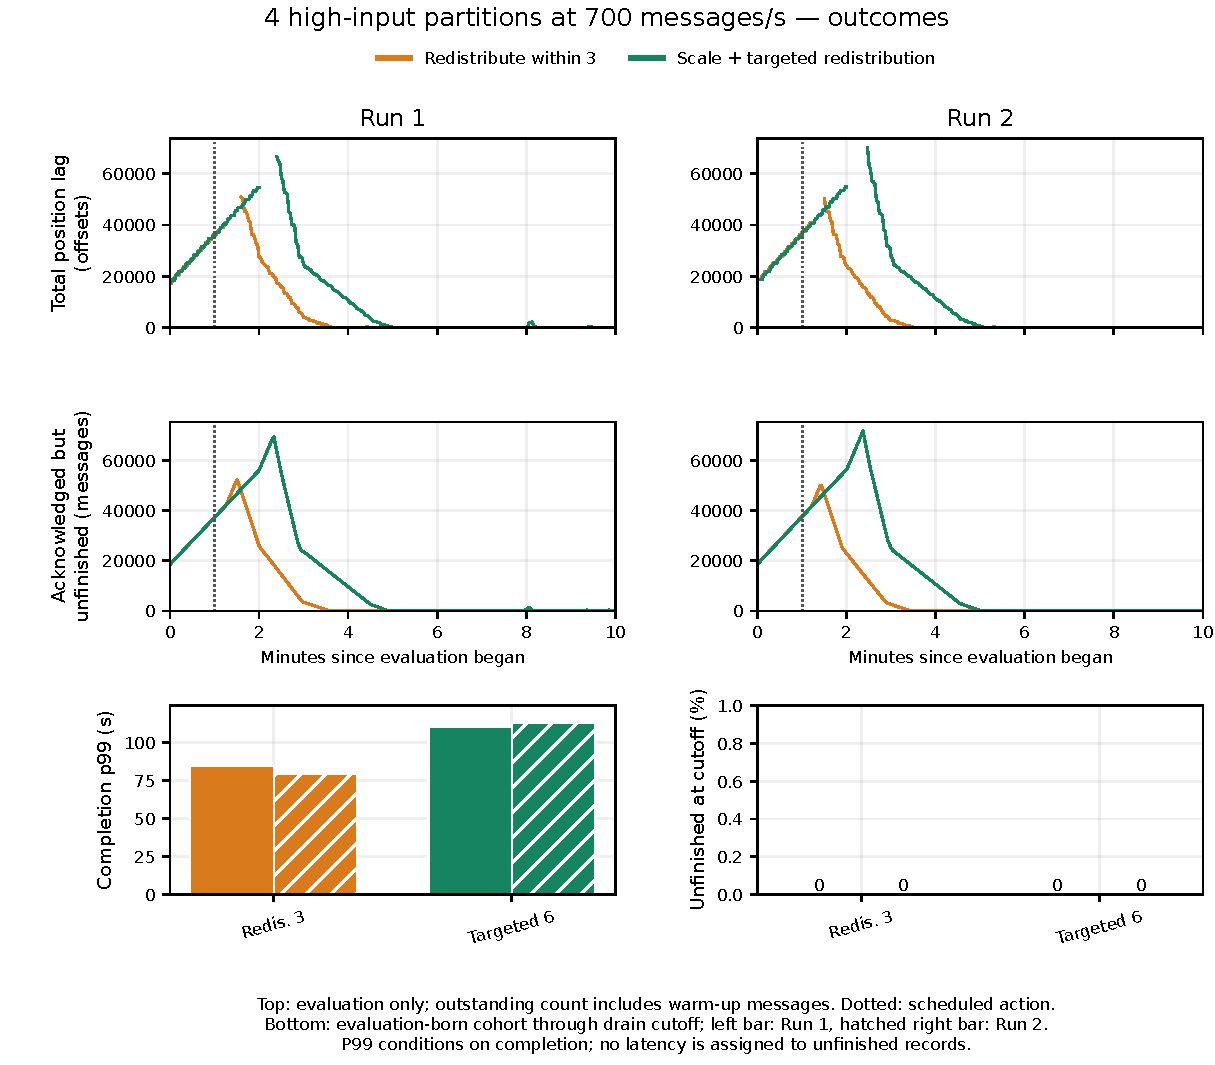
\includegraphics[width=\linewidth,height=.58\textheight,keepaspectratio]{figures/four-partition-compact-outcomes.pdf}
\caption{Outcomes with four high-traffic partitions. The upper panels show total consumer-position lag and acknowledged but unfinished messages during the ten-minute evaluation. The lower panels show p99 for completed evaluation messages and the unfinished percentage at the drain cutoff. Warm-up work is included in the time-series counts but excluded from the evaluation-message outcomes.}
\label{fig:four-partition-compact-outcomes}
\end{figure}
\clearpage

\begin{figure}[!htbp]
\centering
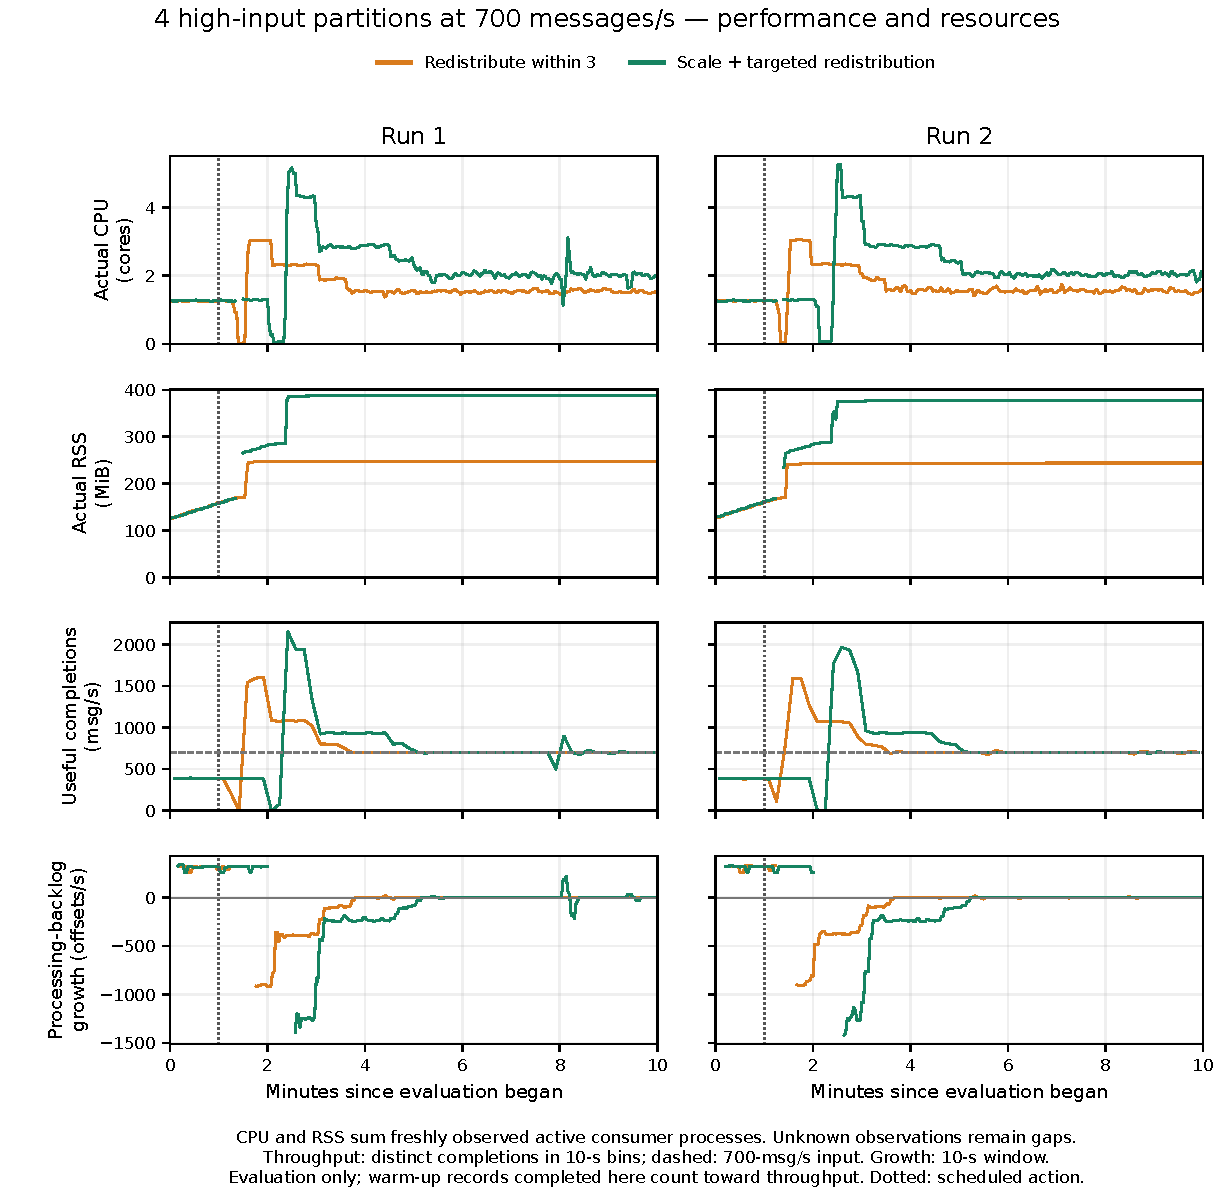
\includegraphics[width=\linewidth,height=.60\textheight,keepaspectratio]{figures/four-partition-compact-performance.pdf}
\caption{Consumer CPU use, resident memory, completion throughput and ten-second processing-backlog growth during the ten-minute evaluation. Resource traces sum fresh measurements for all started consumer processes; an unavailable component leaves a gap. Requested resources and their integrals remain separate in the resource table.}
\label{fig:four-partition-compact-performance}
\end{figure}
\clearpage
\begin{figure}[p]
\centering
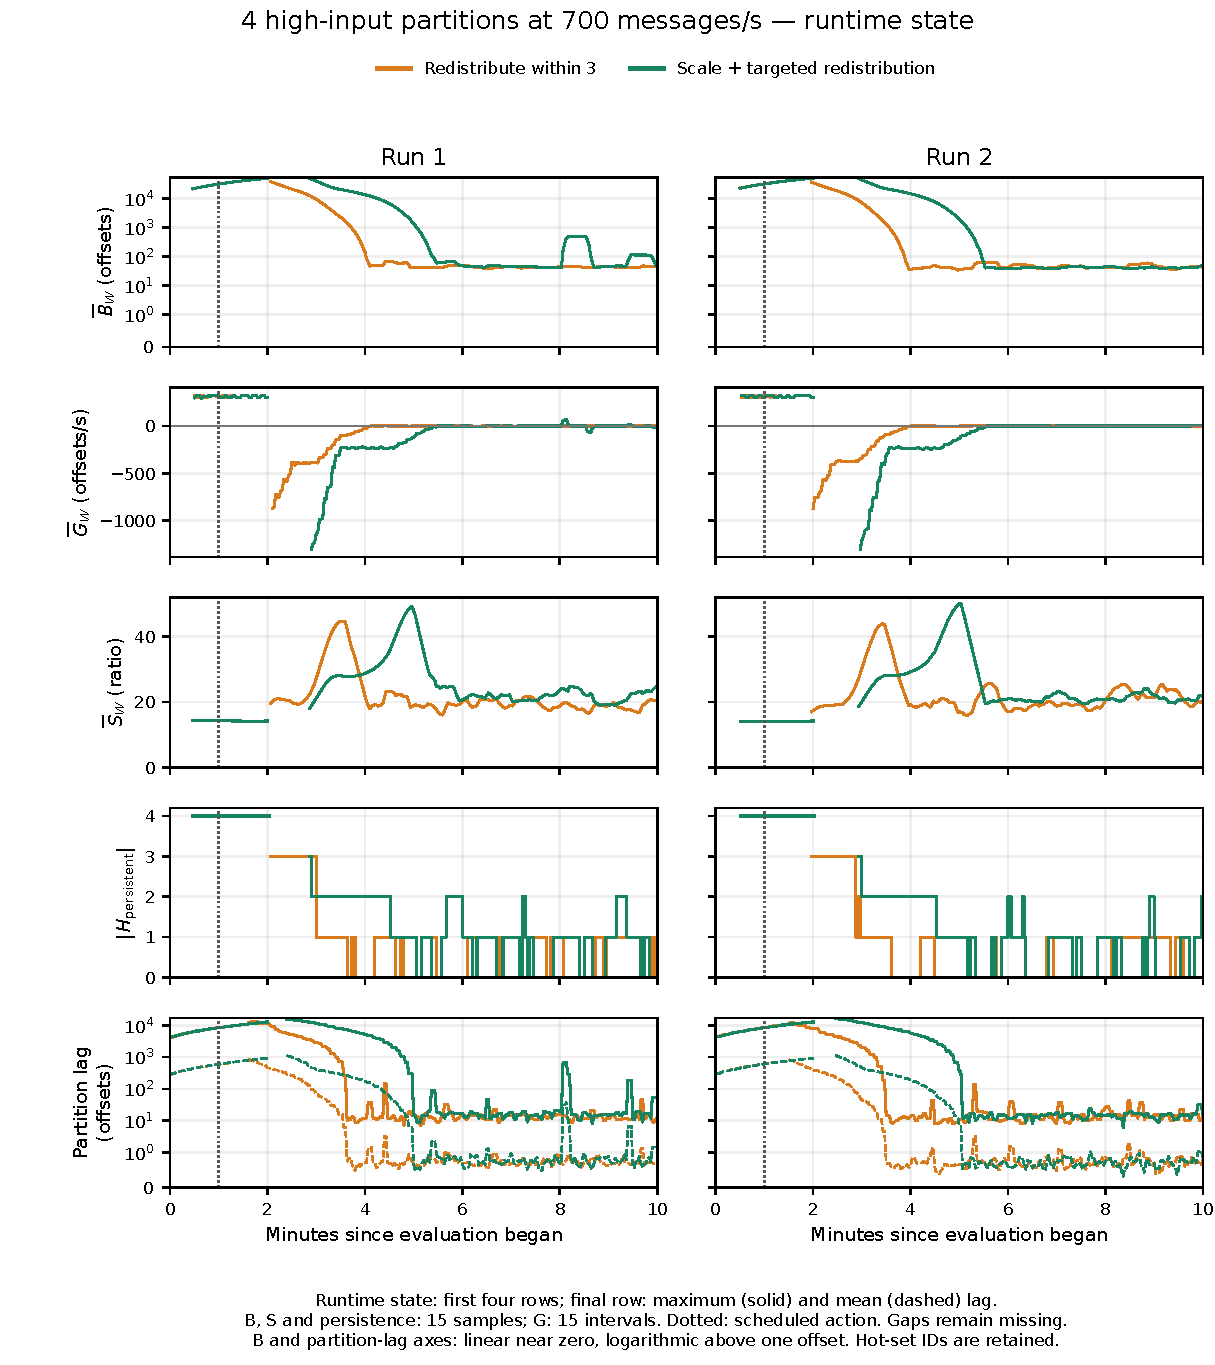
\includegraphics[width=\linewidth,height=.79\textheight,keepaspectratio]{figures/four-partition-runtime-state.pdf}
\caption{Partition-level measurements during the ten-minute evaluation. The first four rows show window-mean total lag, window growth, window-mean skew and persistent-hot count. The final row shows maximum and mean partition lag. Exact persistent-hot identifiers remain in the supporting data; the count alone does not identify a reassignment target. No scheduled action was selected by this reconstructed state.}
\label{fig:four-partition-runtime-state}
\end{figure}
\clearpage
\endgroup
